%%%%%%%%%%%%%%%%%%%%% chapter.tex %%%%%%%%%%%%%%%%%%%%%%%%%%%%%%%%%
%
% sample chapter
%
% Use this file as a template for your own input.
%
%%%%%%%%%%%%%%%%%%%%%%%% Springer-Verlag %%%%%%%%%%%%%%%%%%%%%%%%%%
%\motto{Use the template \emph{chapter.tex} to style the various elements of your chapter content.}
\chapter{Interaction of Particles with Matter}
\label{chap:InteractionsInMatter}

Before more fundamental concepts in the development of the field of nuclear and subnuclear physics are discussed, it is important to introduce fundamental concepts of the interaction of particles in matter. Much of the progress in nuclear, subnuclear and particle physics required ingenious detection techniques of particles. By using just the notions of relativity and scattering theory discussed so far, we will be able to better understand the discoveries that have led to the greater understanding of the nucleus, the nuclear forces and of particles and fundamental interactions in general. 

Understanding particle properties requires particle detectors, and particle detectors are based on the interaction of particles in matter. 

The main properties that will characterize the particles of interest will be quite simple: their mass and kinematic properties and their electric charge. Their spin and magnetic moment will essentially play little role in the following and all the phenomena that will be quantitatively described result from the electromagnetic interaction alone.

It is conceptually simple to measure the momentum of a charged particle using a magnetic field. However, to do so it is important to be able to ``sense'' the presence of a particle and track it as precisely as possible. From the measurement of the momentum of the particle it is less obvious how the mass of the particle can be inferred. For this purpose, all possible properties of the interaction of charged particles in matter will be discussed. How neutral particles can be detected and their energy measured will also be addressed. 

In order to efficiently describe the interaction of particles in matter, this chapter will focus on the loss of energy of particles in matter. The following aspects will be covered.

A charged particle which is crossing a material can lose its energy by:
\begin{itemize}
\item Ionization or excitation of other atoms;
\item Coulomb--scattering with atomic nuclei;
\item Radiation emission in the field of atomic nuclei (\emph{Bremsstrahlung}).
\end{itemize}

A photon interacting with matter can lose its energy via:
\begin{itemize}
\item Photoelectric effect;
\item Compton scattering;
\item Production of electron--positron pairs.
\end{itemize}



\section{The Bohr Atom}
At the end of the XVIII century, experiments had shown
that excited gaseous elements could emit radiation, and different spectral
lines were associated to different elements. Discrete emission lines, with well-defined patterns, were first observed by Johann Balmer in 1885. While Thomson's plum pudding model was coherent with the knowledge of the
time that atoms were known to be electrically neutral and to be composed
of electrons, this model could not provide an explanation for the existence of these lines.

It was really Rutherford's experiment that demonstrated that atoms are composed of positively-charged nuclei, surrounded by electrons. At the time it was already clear that the hypothesis was lacking an explanation for the nature of atomic nuclei: given how small the nuclei seemed to be, how could all the positive charges be kept together against the strong electrostatic repulsion? Well before the secrets of the nucleus were unveiled, the Rutherford model could be used to build more accurate models of the atom.

In 1913, Bohr who had been working with Rutherford, developed his famous atomic model based on the following assumptions:
\begin{itemize}
\item an hydrogen atom is composed by a proton and an electron, kept
  together by the Coulomb potential;
\item the mass of the proton is much greater than the mass of the
  electron;
\item the atom is stationary: electrons revolve in stationary orbits
  around the nucleus and do not radiate energy.
\end{itemize}
Let's assume that the orbits are circular. If $m$ is the mass of the
electron, then
\begin{equation}
  \label{eq:bohr1}
  F=\frac{e^2}{4\pi\epsilon_0 r^2} = m\omega^2 r,
\end{equation}
and the energy of the system is constant and given by:
\begin{eqnarray*}
  E &=& \frac{1}{2}m\omega^2 r^2 - \frac{e^2}{4\pi\epsilon_0 r}\\
    &=& \frac{1}{2}\rr{\frac{e^2}{4\pi\epsilon_0r}} - \frac{e^2}{4\pi\epsilon_0 r}\\
    &=&  -\frac{1}{2}\,\frac{e^2}{4\pi\epsilon_0 r}.
\end{eqnarray*}

Also, if the orbits are stationary, the angular momentum is conserved,
\[L = m\omega r^2 = \text{const}.\]

Bohr introduced the assumption that the angular momentum is quantized,
\[\oint L\ d\phi = n h,\]
where $h$ is the Planck' constant. In another way, one has
\[L = n\hslash = n\frac{h}{2\pi},\]
which fixes the allowed values of the
energy and radius of the electron orbits. From Eq. \eqref{eq:bohr1} we easily get the
quantisation rule for the radius:
\begin{align*}
  m\omega^2r^4 &=\frac{e^2 r}{4\pi\epsilon_0 },\\
  \frac{L^2}{m} &=  \frac{e^2 r}{4\pi\epsilon_0 },\\
  r &\equiv r_n  = \frac{n^2 \hslash^2}{\rr{\frac{me^2}{4\pi\epsilon_0}}},
\end{align*}
where used the subscript $n$ to highlight the fact that the radius $r_n$ is quantised. Similarly, for the energy we have
\[E_n = -m\frac{\rr{\frac{e^2}{4\pi\epsilon_0}}^2}{2n^2\hslash^2}.\]
Bohr's atomic model is also providing an explanation for the lines
appearing in the emission spectrum: lines appear in a discrete number, as a consequence of the quantization of the electronic
orbits. In fact, the wavelength emission is associated with the
 transition of an electron from the $m$-th orbit to the $n$-th orbit ($n<m$), which happens with the emission of a photon with an energy given by
equation:
\[h \nu = E_m - E_n.\]

Let's now introduce two fundamental constants which will be convenient to simplify notation in the theory of nuclear and particle physics. The fist one is the
\emph{fine--structure constant} $\alpha$, defined as
\[\alpha = \frac{e^2}{4\pi\epsilon_0\hslash c} \simeq \frac{1}{137},\]
and the second one is the \emph{classical electron radius} $r_e$, which is defines as
the radius of a charged sphere with electrostatic energy equal to
$m_ec^2$:
\[m_ec^2 = \frac{e^2}{4\pi\epsilon_0 r_e}.\]

Using these definitions, it is possible to write the two formulas for
$E_n$ and $r_n$ in the following way:
\begin{eqnarray*}
  E_n &=& -\frac{1}{2n^2}\alpha^2mc^2,\\
  r_n &=& n^2 \frac{r_e}{\alpha^2}.
\end{eqnarray*}
For the fundamental state of the hydrogen atom, we have
\begin{eqnarray*}
  E_1 &=& -13.6\ \electronvolt,\\
  a &=& r_1 = 0.53\ \times\ 10^{-10}\ \meter.
\end{eqnarray*}

The magnetic moment of a system can be expressed in terms of its angular momentum. If we see a particle as a coil of surface $S$ with a given electric current $i$, for example, its magnetic (dipole) moment will be given by
\begin{equation*}
  \vec{\mu} = i\vec{S}.
\end{equation*}
In the case of Bohr's model, we can calculate the magnetic moment associated to one orbit of the electron, by identifying
\begin{align*}
  \vec{S} &= \pi r^2 \hat{n},\\
  i &= e/T = e \nu = \frac{e\omega}{2\pi},
\end{align*}
where $T$ is the period of the orbit and $\nu=1/T=\omega/2\pi$ its frequency, and $\hat{n}$ is the unit vector orthogonal to the orbit plane. We then get
\begin{equation*}
  \vec{\mu} = \pi r^2 \frac{e{\omega}}{2\pi}\hat{n} = \frac{e\vec{L}}{2m},
\end{equation*}
from which one can define another fundamental constant, the \emph{Bohr magneton}, which is the magnetic moment of the fundamental state of the hydrogen atom:
\begin{equation*}
  \mu_B = \frac{e\hslash}{2m} = 5.8\times 10^{-5}\ \electronvolt / \tesla.
\end{equation*}
The Bohr magneton is naturally used as the unit for expressing the magnetic moment of fundamental particles. The above expression is of course valid only in the international system of units (and remember that here $m$ is the electron mass!).

\section{Energy loss by ionization}
\subsection{The Bohr formula}\label{sec:energyLossBohr}
It is interesting to take a closer look at the derivation of the energy loss of a charged particle in a material using some of the concepts discussed in Chapter~\ref{Scattering-1}.

To do so we consider an atom with $Z$ electrons and a nucleus with a
charge equal to $Ze$, and an interacting particle with charge $ze$ and mass $M$ typically larger than the mass of the electron $m_e$. A picture of the interaction of the particle with an electron of the atom is given in Fig.~\ref{fig:passRadMat1}. 

\begin{figure}
  \centering 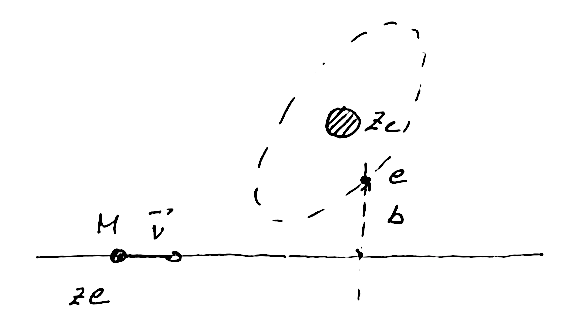
\includegraphics[width=0.5\textwidth]{passRadMat1.png}
  \caption{Illustration of the interaction of a particle of mass $M$ and charge $ze$ with an electron of an atom with atomic number $Z$. The impact parameter of the interaction is $b$.}
  \label{fig:passRadMat1}
\end{figure}

The most efficient way to compute the energy loss is to express the system in the frame where the particle of mass $M$ is at rest and the electron travels towards it, as illustrated in Fig.~\ref{fig:passRadMat2}. From the fundamental principle of dynamics, the total amount of momentum transferred to a 
single electron of the atom can be expressed as a function of the Coulomb force generated by the charge $ze$:

\[ \Delta \vec{p} = \int_{-\infty}^{+\infty}\vec{F_C}\ dt,\] where $F_C$ is due to the Coulomb potential, and can be expressed as

\[F_C =\frac{ze^2}{4\pi\epsilon_0r^2}.\]

\begin{figure}
  \centering 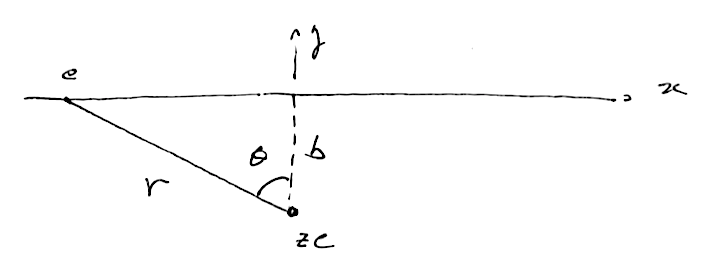
\includegraphics[width=0.5\textwidth]{passRadMat2.png}
  \caption{Illustration of the reference frame in which the particle with mass $M$ is at rest and the atomic electron travels towards it.}
  \label{fig:passRadMat2}
\end{figure}

We can then consider the two main projections of the momentum transfer, where the first is the one along the direction of motion of the electron, i.e. $\Delta\vec{p}$ along the $x$-axis (the direction of motion!) of Fig. \ref{fig:passRadMat2}:

\begin{eqnarray*}
  \Delta p_{\parallel} &=& \int_{-\infty}^{+\infty} \frac{ze^2}{4\pi\epsilon_0}\frac{1}{x^2+b^2}\sin\theta\ dt,\\
                       &=& \int_{-\infty}^{+\infty} \frac{ze^2}{4\pi\epsilon_0}\frac{1}{x^2+b^2}\sin\theta\ \frac{dx}{v},
\end{eqnarray*}
in which we used $dt = dx / v$, and $\theta$ is the angle between the vector $\vec{r}$ and the $y$-axis. Let's assume $v = \text{const}$ and
write
\[\sin\theta = \frac{x}{\sqrt{x^2+ b^2}},\]
so that
\[\Delta p_{\parallel} = \frac{ze^2}{4\pi\epsilon_0v}\int_{-\infty}^{+\infty}\frac{x}{\rr{x^2+b^2}^{\frac{3}{2}}} dx.\]
Now, we use $r = \sqrt{x^2 + b^2}$, with
\begin{eqnarray*}
  \od{r}{x} &=& \frac{1}{2}\frac{2x}{\sqrt{x^2+b^2}}=\frac{x}{r},\\%\frac{x}{\sqrt{x^2+b^2}}\\
  r\,dr &=& x\,dx,
\end{eqnarray*}
from which we get
\begin{eqnarray*}
  \Delta p_{\parallel} &=& \frac{ze^2}{4\pi\epsilon_0v}\int_{-\infty}^{+\infty}\frac{r}{r^3} dr \\&\propto& \int_{-\infty}^{r_0} \frac{1}{r^2}\ dr - \int_{r_0}^{+\infty}\frac{dr}{r^2}\\
             &=& \qq{-\frac{1}{r}}_{-\infty}^{r_0} - \qq{-\frac{1}{r}}_{r_0}^{+\infty} = \qq{-\frac{1}{r}}_{r_0}^{+\infty} - \qq{-\frac{1}{r}}_{r_0}^{+\infty} =0.
\end{eqnarray*}
This shows that the transferred momentum along the x--axis,
i.e. parallel to the direction of the incoming particle, is zero. 

Instead, the component along the $y$-axis, i.e. the orthogonal direction with respect to the direction of motion, can be computed as:
\begin{eqnarray*}
  \Delta p_{\perp} &=& \int_{-\infty}^{+\infty} \frac{ze^2}{4\pi\epsilon_0} \frac{1}{\rr{x^2+b^2}}\cos\theta\frac{dx}{v} \\
             &=&  \frac{ze^2}{4\pi\epsilon_0v} \int_{-\infty}^{+\infty} \frac{1}{b^2}\cos^3\theta dx,
\end{eqnarray*}
in which we used
\[ \cos^2\theta = \frac{b^2}{x^2+b^2}.\]

Now let's compute the integral in $d\theta$:
\begin{eqnarray*}
  x^2 + b^2 &=& \frac{b^2}{\cos^2\theta},\\
  x^2 &=& \frac{b^2\rr{1-\cos^2\theta}}{\cos^2\theta} = b^2\tan^2\theta,\\
  x &=& b\tan\theta,\\
  \od{x}{\theta} &=& \frac{b}{\cos^2\theta},
\end{eqnarray*}
which gives
\begin{eqnarray*}
  \Delta p_{\perp} &=& \frac{ze^2}{4\pi\epsilon_0 vb}\int_{-\frac{\pi}{2}}^{+\frac{\pi}{2}}\cos\theta\ d\theta\\
             &=& \frac{ze^2}{4\pi\epsilon_0 vb} \cdot 2.\\
\end{eqnarray*}
This last equation can simply be written as
\[\Delta p_{\perp} =  \frac{ze^2}{4\pi\epsilon_0 b^2} \cdot \frac{2b}{v}.\]
This means we can see the overall momentum transfer as the momentum transferred by a constant force $ze^2/4\pi\epsilon_0 b^2$ for a time equal to $2b/v$. The "average force" is simply the Coulomb force from a charge $ze$ at a distance equal to the impact parameter, and the time defines the {\bf scattering time}.

An important note at this point is that the trajectory of the electron is assumed essentially to be a straight line, which is clearly an approximation. This approximation holds only in the case where the velocity of the particle of mass $M$ is large enough with respect to the velocity of the electron in its orbit. For this specific calculation we will focus on a very specific energy range of the incident particle: the one where the velocity is large enough to make this approximation valid, but still not too large to break the assumption of a non-relativistic regime.

Since $\Delta p_x = 0$, the only contribution to the energy
transferred to the electron comes from the perpendicular momentum change. In the non-relativistic case, the kinetic energy loss can be written as
\[\Delta E\rr{b} = \frac{\Delta p^2}{2 m_e} = \frac{2z^2e^4}{m_e v^2 \rr{4\pi\epsilon_0}^2b^2},\]
where we highlighted the fact that the energy depends on the impact parameter.
It should be emphasized that the velocity here is non-relativistic in order to be able use the above energy-momentum relation.
While the regime is non-relativistic in this case, we will still express the formula in terms of the velocity normalised to the speed of light $\beta = v/c$: substituting the equation of the classical radius of the electron, the energy loss becomes
\begin{eqnarray*}
  \label{eq:bohr2}
  \Delta E\rr{b} &=& \frac{2z^2e^4}{m_e\beta^2c^2 \rr{4\pi\epsilon_0}^2 b^2}\\
                 &=& \frac{2z^2m_e c^2}{\beta^2 b^2}\qq{\frac{e^2}{4\pi\epsilon_0m_ec^2}}^2\\
                 &=& \frac{2z^2m_e c^2}{\beta^2 b^2}r_e^2.
\end{eqnarray*}

The energy transferred to a single electron of the atom from a particle of mass $M$ and charge $ze$ can thus be written as
\begin{equation}
  \label{eq:bohr3}
 \boxed{ \Delta E = 2m_ec^2\frac{z^2}{\beta^2}\frac{r_e^2}{b^2}.}
\end{equation}

In the reference frame of the interacting particle, the material it encounters can be seen as  a ``beam'' of
electrons moving towards it. The goal is to compute the energy loss per unit path length of the particle: in order to do so, we will express the energy loss as a function of the impact parameter and we will need to start by taking into account all the electrons with a given impact parameter within the ``beam''. 

If $n_e$ is the electron density in
the material (number of electrons per unit volume), then the number of electrons in an element path of the particle $dx$ and with a given impact parameter $b$ will define a cylindrical region around the charge, as shown in Fig. \ref{fig:passRadMat3}, with volume $V$. The number of interacting points with an impact parameter $b\in\qq{b,b+db}$, $dN_I$, will therefore be:
\[dN_I = n_e V = n_e\ 2\pi b\ db dx.\].

\begin{figure}
  \centering 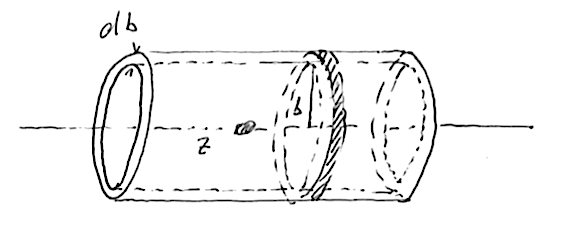
\includegraphics[width=0.5\textwidth]{passRadMat3.png}
  \caption{Illustration of the element cylindrical volume defined for a given impact parameter $b$. }% ,around the charge ze,which volume is given by the formula $2\pi b\ db dx\$ } 
  \label{fig:passRadMat3}
\end{figure}

The absolute value of the element energy loss in the infinitesimal path length $dx$ at a given impact parameter $b$ within an infinitesimal element impact parameter $db$ can then be expressed as follows: 

\[\frac{d^2E}{dxdb} = n_e r_e^2 m_e c^2 \frac{4\pi}{b}
  \frac{z^2}{\beta^2},\]
where we multiplied Eq. \eqref{eq:bohr3} by $dN_I$.
  
In order to compute the energy loss per element path length $dE/dx$, we must integrate the above formula with respect to $b$. This is in principle a clearly divergent integral:
\[\frac{dE}{dx} = n_e r_e^2 m_e c^2 4\pi
  \frac{z^2}{\beta^2} \int_{b_\text{min}}^{b_\text{max}}\frac{db}{b} = n_e r_e^2 m_e c^2 4\pi
  \frac{z^2}{\beta^2} \ln \frac{b_\text{max}}{b_\text{min}} \]
Is it worrisome? No, because the range of possible impact parameters $b$ is necessarily limited. To estimate the energy loss, reasonable estimates of the values of $b_\text{min}$ and $b_\text{max}$ need to be made.

\begin{itemize}
\item The scattering time has to be relatively small as discussed above in order for the electron not to be moving significantly in its atomic orbit during the scattering time. A natural limit in the scattering time will therefore be the revolution period of the electron around the atom, which in the reference frame of the electron is $T_e = 1/\langle \nu_e\rangle$, where 
  $\langle v_e \rangle$ is the average orbital frequency of electrons. As the scattering time could be expressed as approximately $b/v$, then we require that it does not exceed the time needed
  for an electron to complete an orbital revolution. We take into account the time dilation of the revolution period when seen by the moving particle, $\gamma T_e = \gamma /\langle \nu_e\rangle$. As a consequence, $b_\text{max}$ is expressed as 
  \[b_\text{max} = \frac{\gamma v}{\langle v_e \rangle} = \frac{\beta \gamma c}{\langle v_e \rangle}.\]

\item According to the uncertainty principle, 
$$ \Delta p_e  \Delta x > \frac{\hslash}{2}. $$
If the momentum transferred to the electron is equal to the momentum of the electron itself, i.e. $\Delta p_e \sim p_e = m_e \gamma \beta c$, the minimum allowed spatial ``resolution'' $\Delta x$ for the electron position can be taken as $\Delta x = b_\text{min}$, i.e.
  \[b_\text{min} \sim \frac{\hslash}{p_e} = \frac{\hslash}{m_e\beta\gamma c}.\]
\end{itemize}

Having defined the bounds for the integration, the density of electrons in a material can be defined assuming an isotropic material with density $\rho$ [g/cm$^3$], atomic mass $A$ [g/mol$^{-1}$] and atomic number $Z$ [$\#e^-$/atom] using the Number of Avogadro $\mathcal{N}_A$ [mol$^{-1}$] as:
\[n_e = \frac{\mathcal{N}_A Z \rho}{A} \; \; {[\#e^-/\si{cm^{3}}]},\] 
and finally we get
\begin{eqnarray*}
  \od{E}{x} &=& \int_{b_{\min}}^{b_{\max}} 4\pi n_e r_e^2m_e c^2\frac{z^2}{\beta^2}\frac{db}{b}\\
             &=& 4\pi  \frac{\mathcal{N}_A Z \rho}{A} r_e^2m_e c^2\frac{z^2}{\beta^2}\qq{\ln\frac{b_{\max}}{b_{\min}}},\\
\end{eqnarray*}
which gives the expression for Bohr's formula of energy loss of a charged particle traveling in a material:
\begin{equation}
 \boxed{ \der{E}{x} = 4\pi r_e^2m_ec^2\,\frac{\mathcal{N}_A Z\rho}{A}\,\frac{z^2}{\beta^2}\,\ln\frac{m_ec^2\beta^2\gamma^2}{\hslash\langle v_e\rangle }.}
\end{equation}

This approximate estimate of the energy loss of a charged particle in a material has a quite limited kinematic range. A more extended formulation is given in the following section: it will be interesting to note that the two formulations are surprisingly close.

\subsection{The Bethe-Bloch formula}
A more general expression of the energy loss, which is valid also in the relativistic regime and which takes into account more intricate quantum effects has been derived in 1930 by Hans Bethe in the non relativistic regime and then deriving a relativistic correction in 1932. The equation was later completed by Felix Bloch in 1933, who introduced a specific additional term. 

While Bohr's approach was fully classical, Bethe took an quantum-mechanical approach which he extended in the relativistic regime. While a full derivation is beyond the scope of these lectures, we will introduce the Bethe equation from the relation between the energy loss and the impact parameter obtained  from energy-momentum dispersion relation, Eq.~\eqref{eq:bohr3}, yielding
\[ \frac{\Delta E_\text{max}}{\Delta E_\text{min}} =  \frac{b_\text{max}^2}{b_\text{min}^2}.\]
Here it should be noted that the maximal energy transfer will correspond to the minimal impact parameter and vice-versa,  i.e. that \(\Delta E_{max} \propto 1/b_{min}^2\) and \(\Delta E_{min} \propto 1/b_{max}^2\), thus giving the expression above.

The absolute value of energy loss can be expressed in terms of the ratios of the square-root of the maximum and minimal energy losses, which will translate to the logarithm of the ratio divided by $2$: 

\[\frac{dE}{dx} = \frac{\mathcal{N}_A Z \rho}{A} r_e^2 m_e c^2 4\pi
  \frac{z^2}{\beta^2} \frac{1}{2} \log \frac{\Delta E_{max}}{\Delta E_{min}}. \]

We will start from the maximal energy transfer $\Delta E_\text{max}$ from a kinematic standpoint and just consider a two-body scattering of the particle with mass $M$ and charge $ze$ on the electron, which is initially at rest, and compute the maximum kinetic-energy transfer. Let
$\vec{p}$ and $\vec{p}_1$ be, respectively, the momentum of the
particle before and after the scattering, and $\vec{p}_2$ the electron
momentum in the final state, as shown in Fig.~\ref{fig:passRadMat4}.

\begin{figure}
  \centering 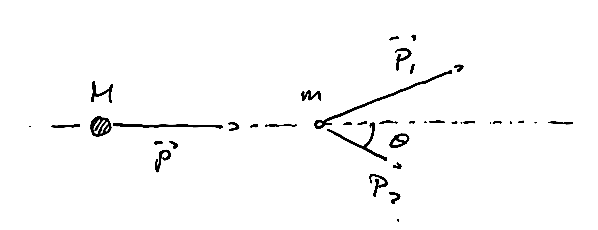
\includegraphics[width=0.5\textwidth]{passRadMat4.png}
  \caption{Illustration of the scattering of a particle with mass $M$ on an electron at rest, used for the computation of the maximum energy loss of the particle (i.e. the maximum kinetic-energy transfer to the electron). The angle $\theta$ is the angle between the momentum of the electron after the scattering and the original direction of the incoming particle.}
  \label{fig:passRadMat4}
\end{figure}

Momentum and energy conservation laws can be written as:
\begin{eqnarray*}
  \vec{p} &=& \vec{p}_1 + \vec{p_2},\\
  E + mc^2 &=& E_1 + E_2.\\
\end{eqnarray*}
From this last equation, using $E^2 = M^2c^4 + p^2 c^2$ and
$p = M \gamma \beta c$:
\begin{eqnarray*}
  E_1 &=& E + mc^2 - E_2,\\
  \qq{M^2c^4 + \vec{p}_1^2c^2}^{\frac{1}{2}} &=& E + mc^2 - E_2,\\
  M^2c^4 + \rr{\vec{p}-\vec{p_2}}^2c^2 &=& \rr{E + mc^2 - E_2}^2,\\
  M^2c^4 + p^2c^2 + p_2^2c^2 -2pp_2c^2\cos\theta &=& E^2 +m^2c^4 +E_2^2\\
      & & +2Emc^2 -2 E_2mc^2 -2EE_2,\\
  -2pp_2c^2\cos\theta &=& 2m^2c^4 +2Emc^2 -2 E_2mc^2 -2EE_2\\
      &=& 2mc^2\rr{mc^2 + E} -2E_2\rr{mc^2 + E}\\
      &=& 2\rr{mc^2 -E_2}\rr{mc^2 + E}.
\end{eqnarray*}
Squaring both terms gives:
\begin{eqnarray*}
  \rr{mc^2+E}^2\rr{E_2^2 + m^2c^4 -2E_2mc^2} &=& p^2p_2^2c^4\cos^2\theta,\\
  \rr{mc^2+E}^2\rr{E_2^2 + m^2c^4 -2E_2mc^2} &=& p^2E_2^2c^4\cos^2\theta - p^2m^2c^6\cos^2\theta.\\
\end{eqnarray*}
Then,
\begin{eqnarray*}
  \qq{\rr{E + mc^2}^2 -p^2c^2\cos^2\theta}E_2^2 & &\\
  -2mc^2 \rr{E+mc^2}^2E_2 & &\\
  +m^2c^4\qq{\rr{E+mc^2}^2+p^2c^2\cos^2\theta} &=& 0.
\end{eqnarray*}
We want to solve this second-order equation for $E_2$. Let's compute the $\Delta/4$:
\begin{eqnarray*}
  \Delta / 4 &=& m^2c^4\rr{E+mc^2}^4\\
             & & - m^2c^4\qq{\rr{E+mc^2}^2+p^2c^2\cos^2\theta}\qq{\rr{E + mc^2}^2 -p^2c^2\cos^2\theta}\\
             &=& m^2c^4p^4c^4\cos^4\theta,\\
  \sqrt{\Delta/4} &=& mc^2 p^2c^2 \cos^2\theta = mc^4 p^2 \cos^2\theta.
\end{eqnarray*}
We finally get to
\[E_2 = mc^2\frac{\rr{E+mc^2}^2 + p^2c^2\cos^2\theta}{\rr{E+mc^2}^2 -
    p^2c^2\cos^2\theta}.\]
This clearly shows that the maximum amount of energy is transferred
when $\cos\theta = 1$, for which the electron energy is
\begin{eqnarray*}
  E_2^{\max} &=&  mc^2\frac{\rr{E+mc^2}^2 + p^2c^2}{\rr{E+mc^2}^2 - p^2c^2}\\
             &=&  mc^2\qq{\frac{E^2+m^2c^4+2Emc^2 + p^2c^2}{E^2+m^2c^4+2Emc^2 - p^2c^2}}\\
             &=&  mc^2\qq{\frac{M^2c^4+m^2c^4+2Emc^2 + 2p^2c^2}{M^2c^4+m^2c^4+2Emc^2}}\\
             &=&  mc^2\qq{1+\frac{2p^2c^2}{M^2c^4+m^2c^4+2Emc^2}}.\\
\end{eqnarray*}
The maximum kinetic energy that can be transferred to the electron is therefore
\[T^{\max} = E_2^{\max} - mc^2 =
  \frac{2mc^2p^2c^2}{M^2c^4+m^2c^4+2Emc^2},\] and if we use $p = Mc\beta\gamma$
and $E = \gamma M c^2$ we get
\[ \boxed{T^{\max} =
  \frac{2m\beta^2\gamma^2c^2}{1+2\gamma\frac{m}{M}+\rr{\frac{m}{M}}^2}.}\]
An useful approximation of this formula in the limit $2\gamma m \ll M$ will be useful for the complete Bethe-Bloch calculation:
\begin{equation}\label{eq:Tmaxapprox}
    \Delta E_{max} = T^{\max} = 2m\beta^2\gamma^2c^2.
\end{equation} 

In order to compute the minimum energy loss of the incoming particle, the intuitive estimate should be the average ionization energy of the electrons of the atom, $\langle I\rangle$. This quantity is non trivial to estimate and was one of the main contributions from Felix Bloch in 1933, who showed that the mean ionization energy can be simply approximated by the relation 

\[\langle I \rangle \sim (10 \, {\rm eV}) \times Z.\]

A similar approximation can be obtained with the Thomas--Fermi model, where $\langle I\rangle $ can be computed from the average ionization energy of hydrogen atoms,
\[\langle I \rangle \sim Z I_H.\]

From the above formula one obtains a formulation of the average ionization energy which depends only on the atomic number $Z$ in units of the electron rest energy (i.e. its mass),

\[ \boxed{\frac{m_e c^2}{I} \sim \frac{3.6 \cdot 10^4}{Z}.}\]

In order to simplify notation, one usually defines the constant $C$ as
\[C = 4\pi r_e^2 m_e c^2 N_A = 0.31\ \frac{\mega\electronvolt}{\gram\cdot\centi\meter^{-2}},\]
and the energy loss formula can then be written as
\begin{equation}
  \frac{1}{\rho}\od{E}{x} = C\,\frac{Z}{A}\,\frac{z^2}{\beta^2}\,\frac{1}{2}\ln\frac{2m_e\gamma^2\beta^2c^2}{I}.
\end{equation}
One often uses $1/\rho\od{E}{x}$ instead of $\od{E}{x}$, in order to highlight the small dependence of the energy loss on the material.

%which, according to the
%1\textsuperscript{st} equation of \ref{eq:bohr2} allows us to get %an
%estimate for $b_{\min}$:
%\[b_{\min} = \frac{ze^2}{\gamma\beta^2m_ec^2\rr{4\pi\epsilon_0}}\]

In fact, by using
\[\frac{m_ec^2}{\langle I \rangle} \sim \frac{3.6\times10^4}{Z},\]
it becomes clear that the energy loss divided by $\rho$ scales as
\[\frac{dE}{\rho dx} \propto \frac{Z}{A}\ln\frac{\text{const}}{Z},\]
which, apart from the density and a logarithmic dependency on $Z^{-1}$, does not depend strongly on the material. If we ignore the logarithmic dependency we obtain that the energy loss per unit of length divided by the density is independent of the material of the detector.

The result of this calculation is often referred to as the Bethe formula. A more precise empirical model for the average ionization energy is obtained from measurements of the ionization energy normalized to the atomic number $Z$, as shown in Fig.~\ref{fig:passRadMat6}. The measurements show a good agreement with the Bloch prediction, with a significant deviation at low $Z$.

\begin{figure}
  \centering 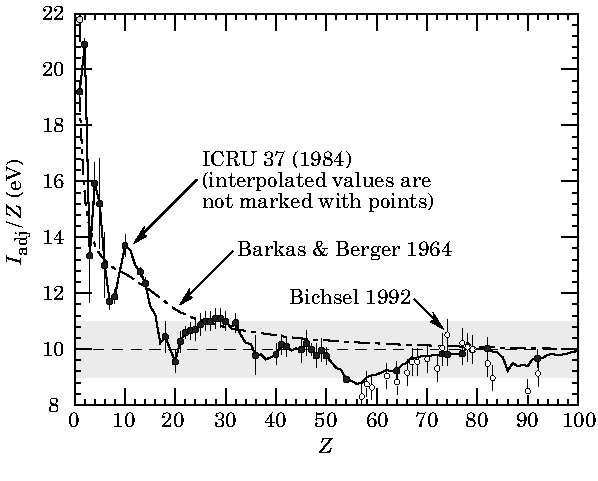
\includegraphics[width=0.75\textwidth]{passRadMat6_Iadj_pegs_adndt}
  \caption{Illustration of the average ionization energy measurement as a function of  the atomic number $Z$. The relation $\langle I \rangle \sim (\SI{10}{eV})\times Z$ is represented by the dashed, horizontal line.}
  \label{fig:passRadMat6}
\end{figure}

A more accurate parameterisation which is valid in a wider range of atomic number \(Z\) is
\begin{eqnarray*}
  \frac{I}{Z} \sim \rr{12 + \frac{Z}{2}}\,\electronvolt &\text{for}& Z \lesssim 10,\\
  \frac{I}{Z} \sim \rr{10 + 60 Z^{-1.2}}\,\electronvolt &\text{for}& Z \gtrsim 10.\\
\end{eqnarray*}

The \(\od{E}{x}\) behaviour described by the Bethe formula is shown in Fig.~\ref{fig:passRadMat8}.

\begin{figure}
  \centering 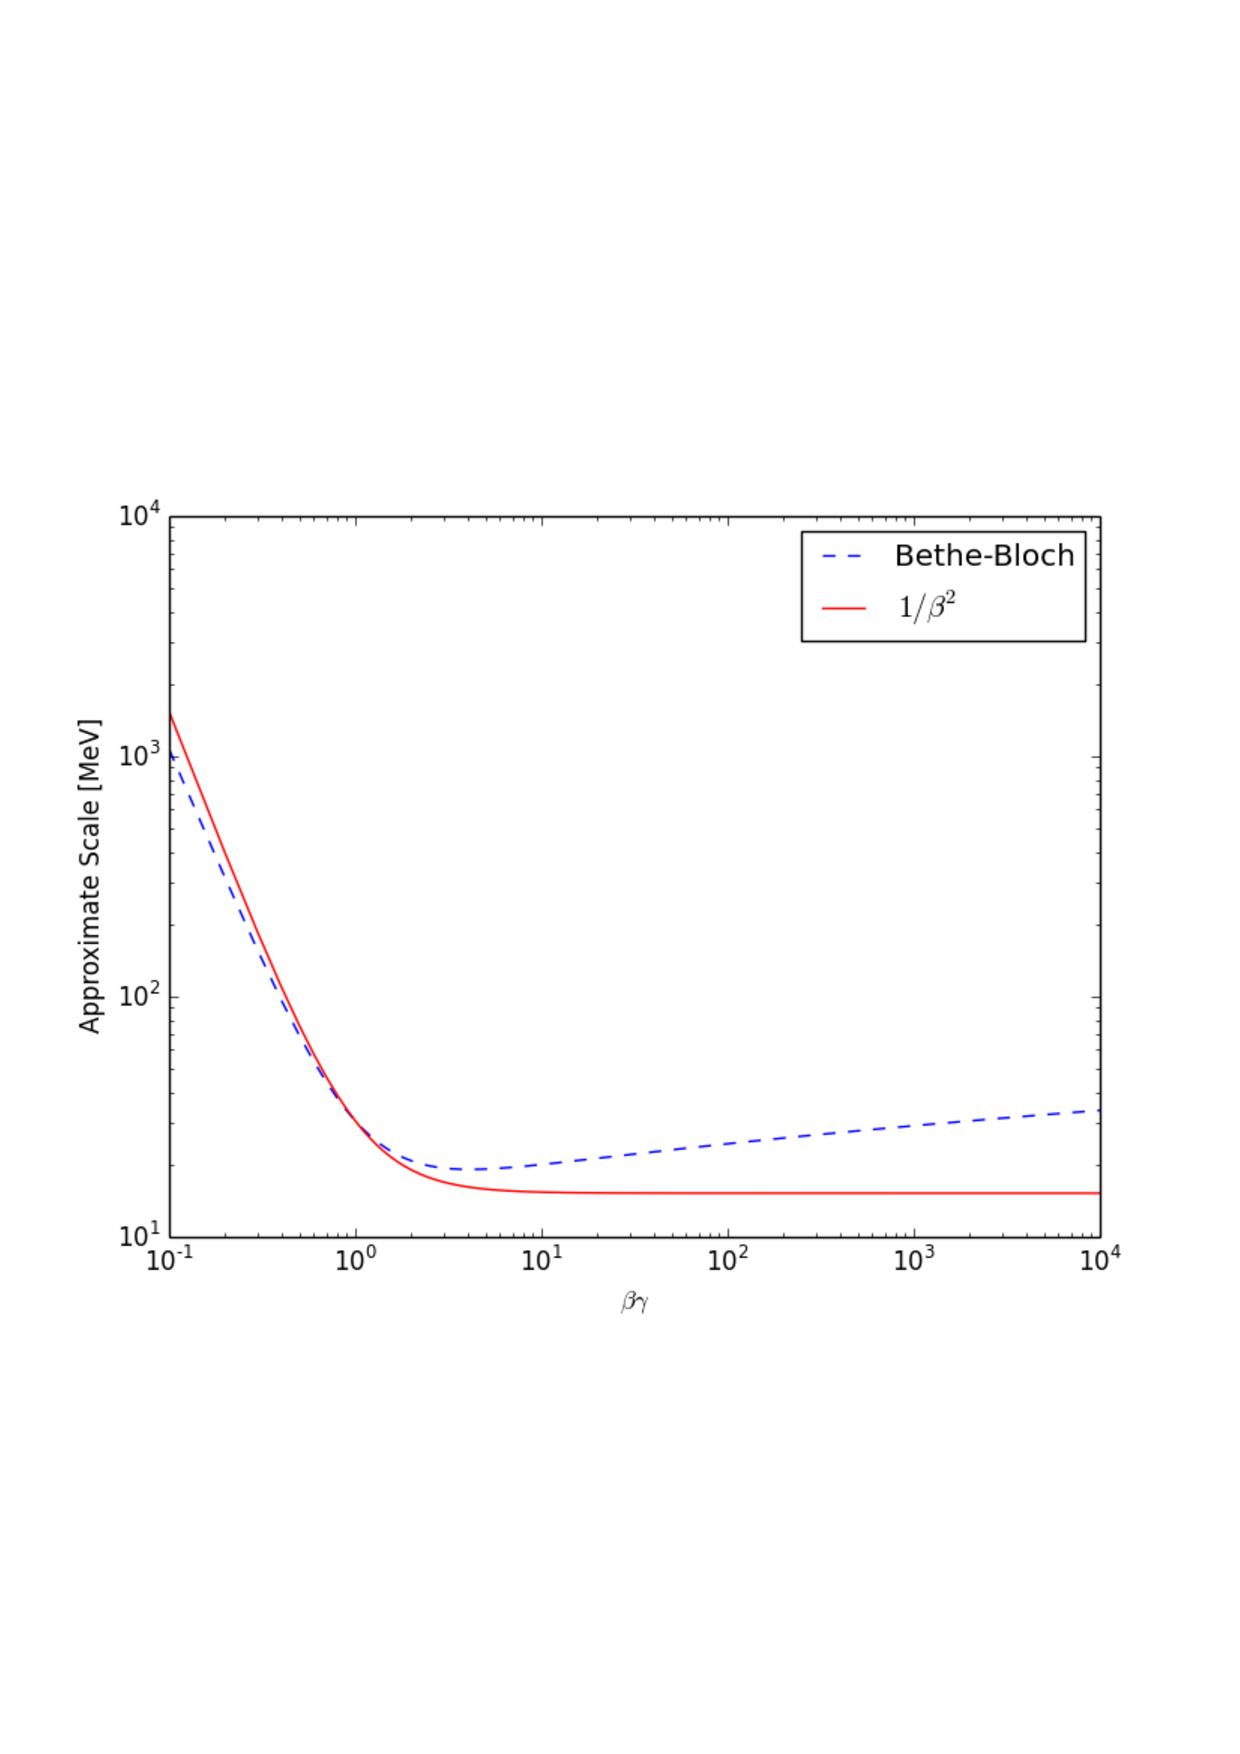
\includegraphics[width=0.75\textwidth]{BetheBloch}
  \caption{Illustration of the behaviour of the energy loss \(\od{E}{x}\) described by the Bethe formula as a function of $\beta \gamma$.}
  \label{fig:passRadMat8}
\end{figure}

\subsubsection{Interpretation}

It is interesting to compare the Bethe formula with the simple dependence in $1/\beta^2$. This shows that in the low energy regime the dominant term  essentially goes as  $1/\beta^2$, indicating that slow particles will lose much more energy by ionization than faster particles. With respect to the simple $1/\beta^2$ behaviour, the Bethe formula shows a slow increase in ionization energy at relativistic velocities, often referred to as \emph{relativistic increase}.

In the higher energy range, compared with the $1/\beta^2$ analytic form, there is a logarithm rise of the energy loss which is interpreted as the increase of the energy loss due to the increase in the electrostatic field "seen" by the probe particle when it is boosted. The electric field components which are orthogonal to the boost axis will be increased by a factor $\gamma$, while the longitudinal component is unchanged.

However, this formulation of the energy loss is incomplete. A more accurate and up-to-date version of the Bethe formula, the Bethe-Bloch formula, is discussed in the next section.

\begin{figure}
  \centering 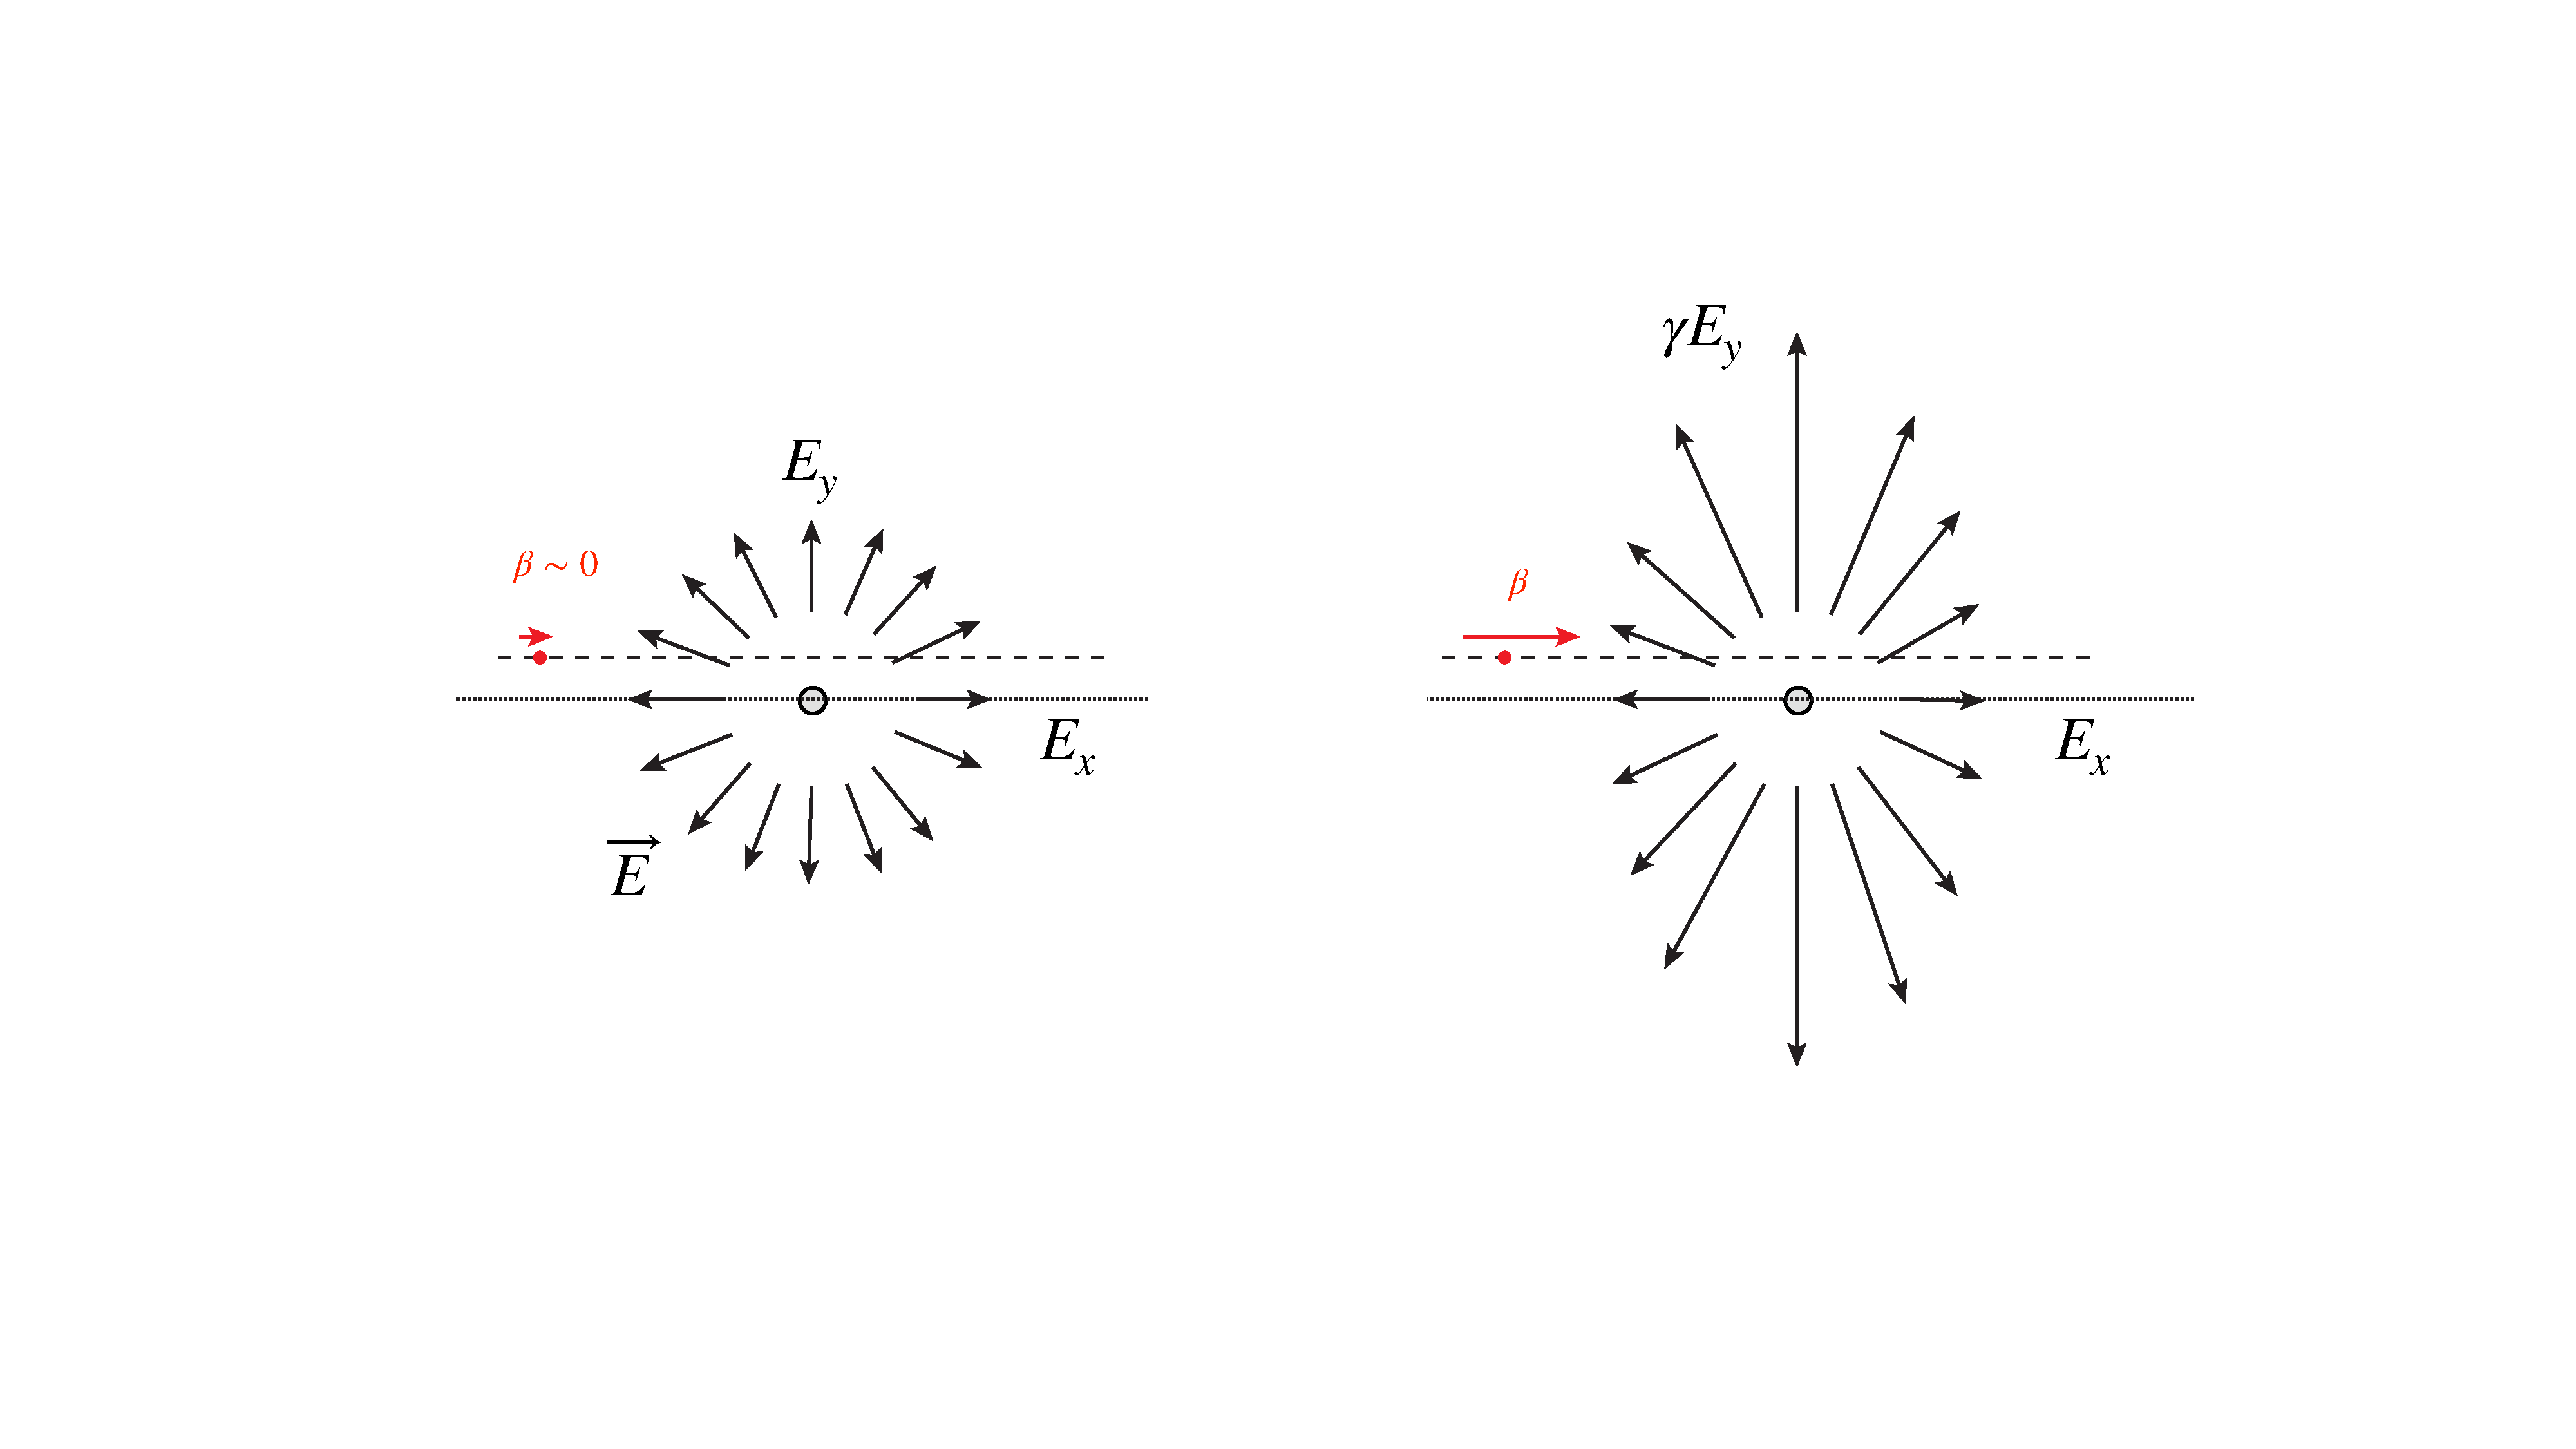
\includegraphics[width=0.8\textwidth]{Field}
  \caption{Illustration of the interpretation of the logarithmic relativistic rise of the energy loss due to the increase of the electric field "seen" by a boosted probe particle.}
  \label{fig:FieldBetheBloch}
\end{figure}


\subsection{The complete Bethe-Bloch formula}
\label{sec:BB} 
The complete Bethe-Bloch formula for the calculation of the energy loss by ionisation, which is valid also in the relativistic regime and takes all known intricate effects into account, is the following:
\[\frac{1}{\rho}\od{E}{x} = Cz^2
  \frac{Z}{A}\frac{1}{\beta^2}\qq{\frac{1}{2}\ln\frac{2m_ec^2\beta^2\gamma^2T_{\max}}{I^2}
    - \beta^2 -\frac{\delta}{2} - \frac{K}{Z}}.\] 
Here $T_{\max}$ corresponds to the maximum kinetic energy which can be transferred to the electrons, as calculated in the previous section. i.e. 
\[T_{\max} = \frac{2m_ec^2\beta^2\gamma^2}{1+2\gamma\frac{m_e}{M} +
    \rr{\frac{m_e}{M}}^2} \xrightarrow{\gamma m_e \ll M}
  2m_ec^2\beta^2\gamma^2,\]and $\delta$ is a term due to the
\emph{density effect} due to the screening of polarisation, which limits the logarithmic growth of
$\od{E}{x}$. The term $K/Z$ is a term which lowers the energy loss for
slowly-moving particles, for which $v$ (and then the kinetic energy
$K$) is not much greater than the electron velocity.\\

\begin{figure}
  \centering 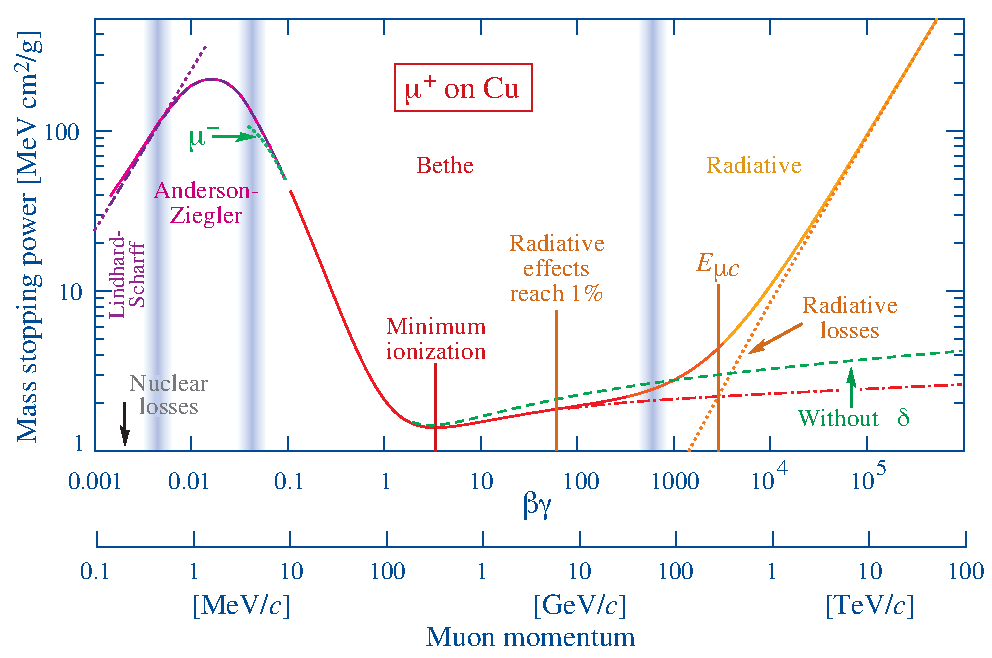
\includegraphics[width=\textwidth]{passRadMat5_rpp_icru49_cu_col}
  \caption{Energy loss normalised to the density of the material ("mass stopping power"), $dE/\rho dx$, for a muon, a particle with a mass of $105 \; \mega\electronvolt$, as a function of its $\beta \gamma$.}
  \label{fig:passRadMat5}
\end{figure}

Figure \ref{fig:passRadMat5} shows on the y--axis the $dE/\rho dx$ of a muon\footnote{Standard model particles will be introduced later in these notes. Here you should consider the muon as a particle identical to the electron, but with a mass of $105 \mega\electronvolt$.} as a function of its momentum. Let's take a look to the region labelled as ``Bethe'' (in which the precision of the formula is around 1\%):
\begin{itemize}
\item at low $\beta$, i.e. at low momentum, the energy loss is dominated by the dependence on $1/\beta^2$;
\item the energy loss has a minimum: particles which are crossing a material such that their energy loss is in this minimum are called \emph{minimally-ionising particles} (MIP); the minimum position is usually at $\beta\gamma \sim 3\div3.5$;
\item after the minimum, the energy loss begins to grow as $2\ln(\beta\gamma)$;
\item in the lowest $\beta\gamma$ region the model is not valid, and empirical models are used to describe the energy loss;
\item in the low $\beta\gamma$ region, the correction $K/Z$ becomes important;
\item for high $\beta\gamma$, the model is no more valid, as the energy loss is dominated by \emph{bremsstrahlung} (described later in this chapter).
\end{itemize}

The correction introduced by $\delta$ is mostly effective at high energy. As the energy of the particle increases, its electric field becomes more flattened and extended, but the real media become polarized, truncating this part of logarithmic rise.

\begin{figure}
  \centering 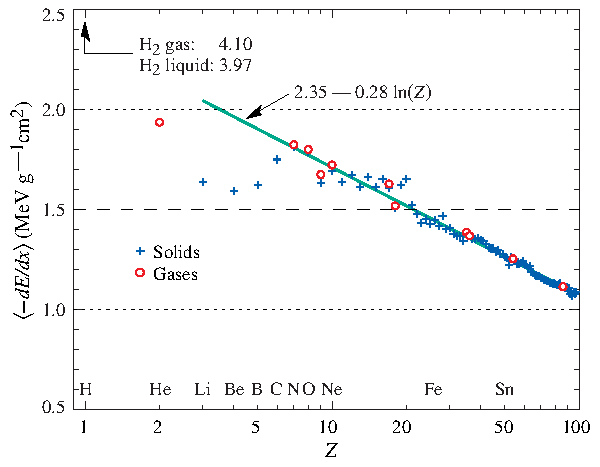
\includegraphics[width=\textwidth]{passRadMat7_dedx_min_06}
  \caption{Value of the energy loss at its minimum (normalised to the  density of the material, $dE/\rho dx$) as a function of the atomic number of different elements ($Z$).
  A linear empirical regression shows that  $dE/\rho dx$ depends on $\ln (Z)$ with a good approximation. }
  \label{fig:passRadMat7}
\end{figure}

Figure \ref{fig:passRadMat7} shows the energy loss at its minimum for different elements. 

Different particles traveling in the same material lose their energy in a similar way. In this case, the Bethe-Bloch law can be seen as
\[-\frac{dE}{dx} = z^2 f(\beta),\]
where $z^2$ multiplies a function of the velocity which is unique for the material.

Since $T=(\gamma-1) Mc^2$, the velocity is a function of $T/M$. This suggests that if the energy loss for a particle with mass $M$ and charge $z$ is known, the energy loss of another particle with mass $M_2$ and $z^2$ will be
\[-\od{E_2}{x} = -\frac{z_2^2}{z_1^2} \od{E_1}{x}\rr{T_2\frac{M_1}{M_2}}.\]

\subsection{Cross Section, Range, Straggling and the Landau Distribution} 
\subsubsection{Cross section}
Equation \ref{eq:bohr3} shows the dependency of $\Delta E$ on the impact parameter $b$. We can compute the cross section of the ionisation energy loss starting from the inverse formula. Let us call $\tilde{E} = \Delta E$ to simplify notation: we have
\[b^2 = \frac{2r_e^2 z^2 m_e c^2}{\beta^2\tilde{E}},\]
and differentiating both members we have
\[|2bdb| = 2r_e^2\,\frac{z^2m_ec^2}{\beta^2}\frac{d\tilde{E}}{\tilde{E}^2},\]
from which we can compute the infinitesimal cross-section in an element cylinder as
\begin{eqnarray*}
  d\sigma &=& \rr{2\pi b} db\\
          &=&2\pi r_e^2 m_e c^2 %n_e
          \frac{z^2}{\beta^2}\frac{d\tilde{E}}{\tilde{E}^2},
\end{eqnarray*}
and finally get the differential cross-section
\[\der{\sigma}{\tilde{E}} = 2\pi r_e^2 m_e c^2 \frac{z^2}{\beta^2}\frac{1}{\tilde{E^2}}.\]
The more energy is lost by the particle, the more collisions are rare.

\subsubsection{Residual Range}
The residual range $R$ is defined as the mean path crossed by a particle in a certain material before losing its entire kinetic energy; it is of course a function of the energy of the particle. Using \(f(E) = -\od{E}{x}\), we have
\begin{eqnarray*}
  R(E) &=& \int_0^R dx \\
       &=& -\int_E^0 \frac{dE}{f(E)}\\
       &=& \int_0^E \frac{dE}{f(E)}.
\end{eqnarray*}
One should note that this quantity is an average quanity: since the energy loss is a stochastic effect, the actual value of $R$ will vary in a certain interval.

In order to measure the residual range it is possible to take an absorber of different length and material and measure the transmission power (ratio of incoming and outgoing particles). Stochastic effects (straggling) are responsible for the smoothed curve of transmission power, as shown in figure \ref{fig:passRadMat8}.

\begin{figure}
  \centering 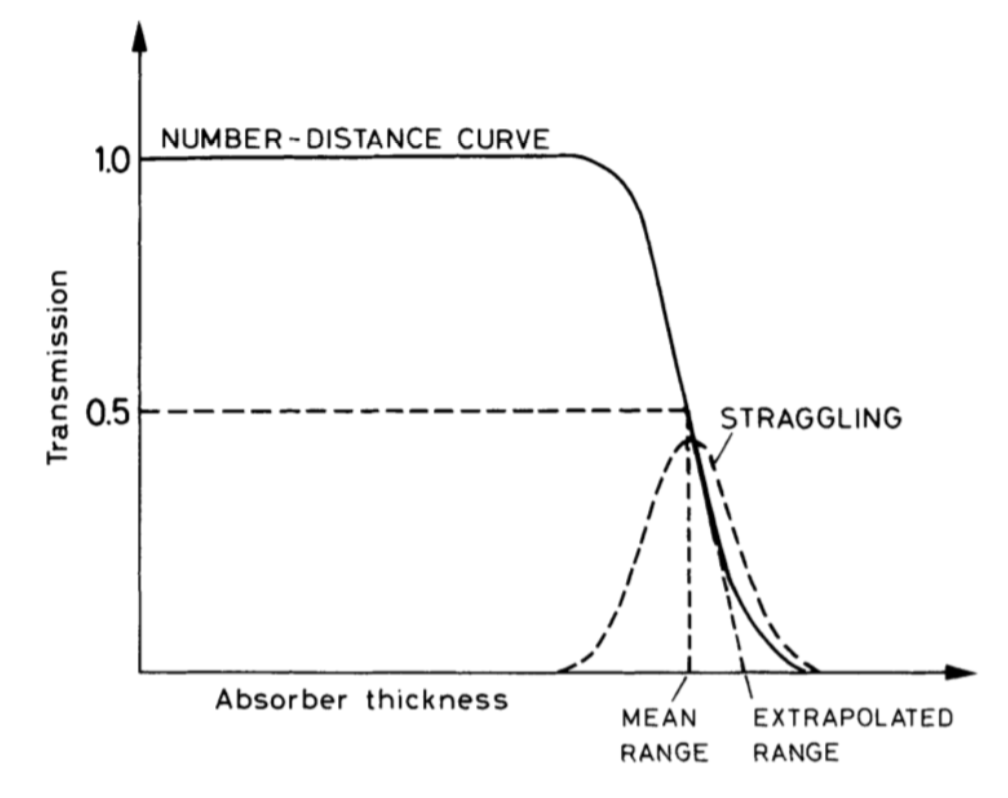
\includegraphics[width=0.6\textwidth]{passRadMat8}
  \caption{Transmission power (fraction of particles in a beam which are transmitted) as a function of the distance traveled by the beam in a given material. Stochastic effects (``straggling'') are responsible for the smoothed curve.
  Note that the average distribution becomes a Gaussian which parameters will be described in Sec. \ref{sec:energystraggling}.
  }
  \label{fig:passRadMat8}
\end{figure}

In order to take into account the effects at low energy loss, it is common to introduce a term like
\[R(E) = R_0(E_{\min}) + \int_{E_{\min}}^E \frac{dE}{f(E)}, \]
which can be measured experimentally, while the integral is computed numerically. Figure \ref{fig:passRadMat9} shows the range divided by $M$ for different particles in different materials. The precision of this prediction is around $1\%$.
\begin{figure}
  \centering 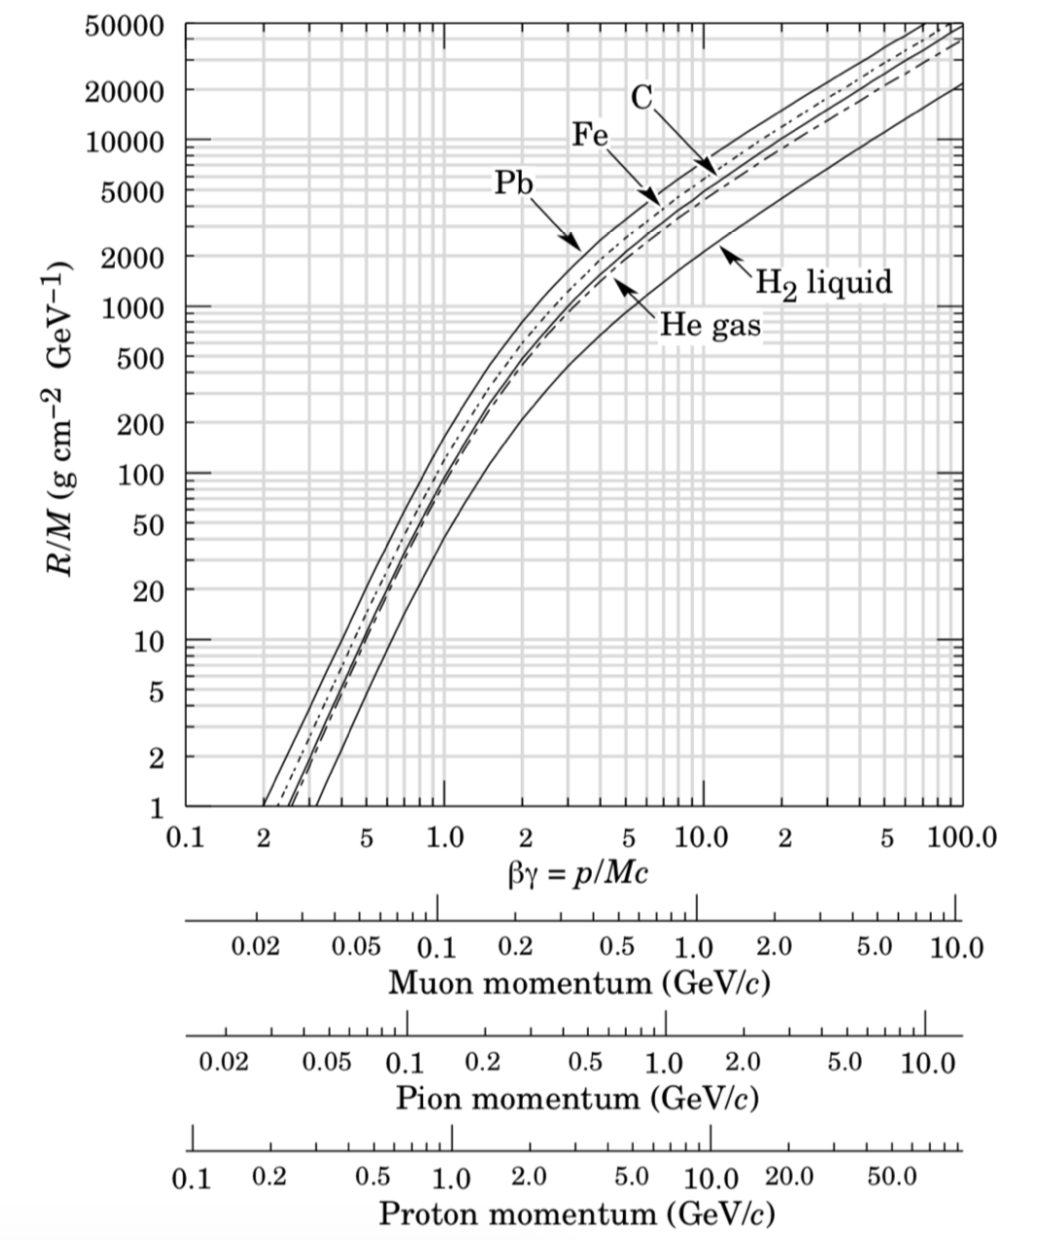
\includegraphics[width=\textwidth]{passRadMat9}
  \caption{Range (times density) of ionizing charged particles ($x \rho$) in liquid  hydrogen, helium gas, carbon, iron, and lead. As an example, for a $K^+$ with mass $\SI{493.7}{MeV/c^2}$ and with momentum \SI{700}{MeV/c}, i.e. $\beta \gamma = 1.42$, from the curves one can read $R/M\sim396$, and so the range is $\SI{195}{g cm^{-2}}$.}
  \label{fig:passRadMat9}
\end{figure}


\subsubsection{Channeling}
Channeling is another limit of Bethe-Bloch formula. If a particle crosses a material at a certain critical angle it is possible that it starts to follow a path in which the number of encountered electrons is lower than  average. This is usually happening at a small angle $\theta_{\text{crit}} \sim 1^\circ$ and $\beta \simeq 0.1$, becoming smaller as the energy rises. Figure \ref{fig:passRadMat10} shows an example of this path.

\begin{figure}
  \centering 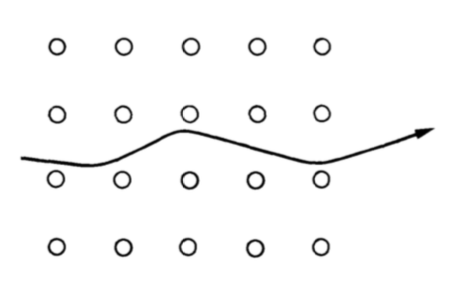
\includegraphics[width=0.5\textwidth]{passRadMat10}
  \caption{Illustration of the phenomenon of channelling, as observed for example in crystals.
  It defines a limit of Bethe Bloch formula.}
  \label{fig:passRadMat10}
\end{figure}

\subsubsection{Energy straggling}\label{sec:energystraggling}
The Bethe-Bloch formula gives an expression of the \emph{average} energy
loss. Since the nature of these interactions is stochastic, the energy
lost by a particle should also be considered as a random variable with a certain distribution.

Although the computation of the energy loss distribution in a material
of length $x$ is difficult (and usually dealt with computer simulation), we will see the limits of very thin and
very thick material.\\

For a \emph{thick material}, we can assume that the energy lost in a single
collision, $\Delta$, is much smaller than the energy of the incoming particle. If
we also assume that this $\Delta$ is small enough  not to change the
$\beta$ of the particle, the central limit theorem ensures us that the
distribution of energy lost by the particle will be Gaussian,
\[f(\Delta) \propto e^{-\frac{\rr{\Delta -
        \bar{\Delta}}^2}{2\sigma^2}},\]
whose expectation value and standard deviation we wish to calculate.
        
The number of collisions in a
length $dl$ with transferred energy
$\tilde{E}\in\qq{\tilde{E},\tilde{E}+d\tilde{E}}$ is
\begin{eqnarray*}
  f(\tilde{E})d\tilde{E} dl &=& \frac{N_A Z \rho}{A} dl \frac{d\sigma}{d\tilde{E}}d\tilde{E}\\
                            &=& \frac{N_A Z\rho}{A} 2\pi r_e^2 m_e c^2 \frac{z^2}{\beta^2}\frac{d\tilde{E}}{\tilde{E}^2}dl\\
                            &=& \frac{C}{2}\frac{Z\rho}{A}\frac{z^2}{\beta^2}\frac{d\tilde{E}}{\tilde{E}^2}dl.
\end{eqnarray*}
If we assume that $\beta$ is constant and neglect the $K/Z$ and density effect corrections, the integral of the Bethe-Bloch
can be easily computed,
\[\int_0^x \frac{dE}{\rho dx} dx = C
  \frac{Z}{A}\frac{z^2}{\beta^2}\frac{1}{2}\rr{\ln\frac{2m_ec^2\beta^2\gamma^2}{I}
    -\beta^2}x,\]
which gives $\bar\Delta$,
\[\bar\Delta = \xi\rr{\ln\frac{2m_ec^2\beta^2\gamma^2}{I} - \beta^2},\]
where we used
\[\xi = \frac{C}{2}\frac{Z}{A}\frac{z^2}{\beta^2}x.\]

The variance can be obtained from its definition:
\begin{eqnarray*}
  \sigma^2 &=& \int f(\tilde{E})\tilde{E}^2d\tilde{E}dl\\
           &=& \int d\tilde{E} dl \frac{C}{2} \frac{Z\rho}{A}\frac{z^2}{\beta^2}\\
           &=&  \frac{C}{2} \frac{Z\rho}{A}\frac{z^2}{\beta^2} \rr{E^{\max} - E^{\min}}x\\
           &\simeq&  \frac{C}{2} \frac{Z\rho}{A}\frac{z^2}{\beta^2}T^{\max}x\\
           &=&  \frac{C}{2} \frac{Z\rho}{A}\frac{z^2}{\beta^2}2m_ec^2\beta^2\gamma^2 x\\
           &=&  C\frac{Z\rho}{A}z^2m_ec^2\gamma^2 x,\\
\end{eqnarray*}
where we replaced $T^{\max}$ with its approximation for $2\gamma m<<M$ from Eq. \eqref{eq:Tmaxapprox}. \\

For a \emph{thin material} we cannot apply the central limit theorem: the
Gaussian approximation will fail, as interactions between particles are rare. In this case, the fluctuations in the energy loss will follow the Landau distribution with a most probable value $\Delta_p < \bar\Delta$:
\[f(\lambda) = \frac{1}{\sqrt{2\pi}} e^{-\frac{\rr{\lambda + e^{-\lambda}}}{2}},\]
where
\[ \lambda = \frac{\Delta - \Delta_p}{\xi}.\]
Other laws which are describing different regions exists. An example of straggling function is shown in Fig. \ref{fig:passRadMat11}.
\begin{figure}
  \centering 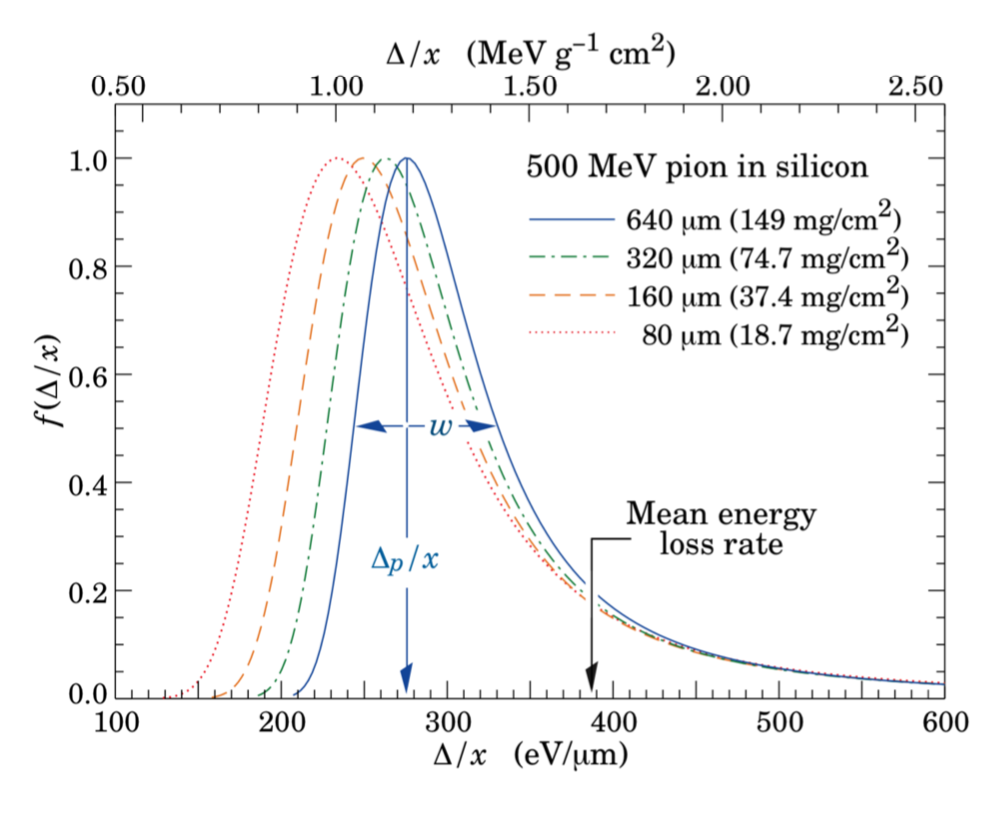
\includegraphics[width=\textwidth]{passRadMat11}
  \caption{Illustration of the Landau distribution modelling the energy loss $\Delta$ over a small distance $x$ travelled by \SI{500}{MeV} pions in silicon.}
  \label{fig:passRadMat11}
\end{figure}


\subsection{Interpretation and Particle Identification} 
As shown in figure \ref{fig:passRadMat12} the energy loss at its minimum is around $1\div2\, \mega\electronvolt\,\gram^{-1}\centi\meter^2$. This corresponds, for a medium with $\rho \sim 10\, \gram\centi\meter^{-3}$ like copper, to a mean energy loss per $1\,\centi\meter$ of \SI{16}{MeV}, i.e. a non--negligible amount of energy.


\begin{figure}
  \centering 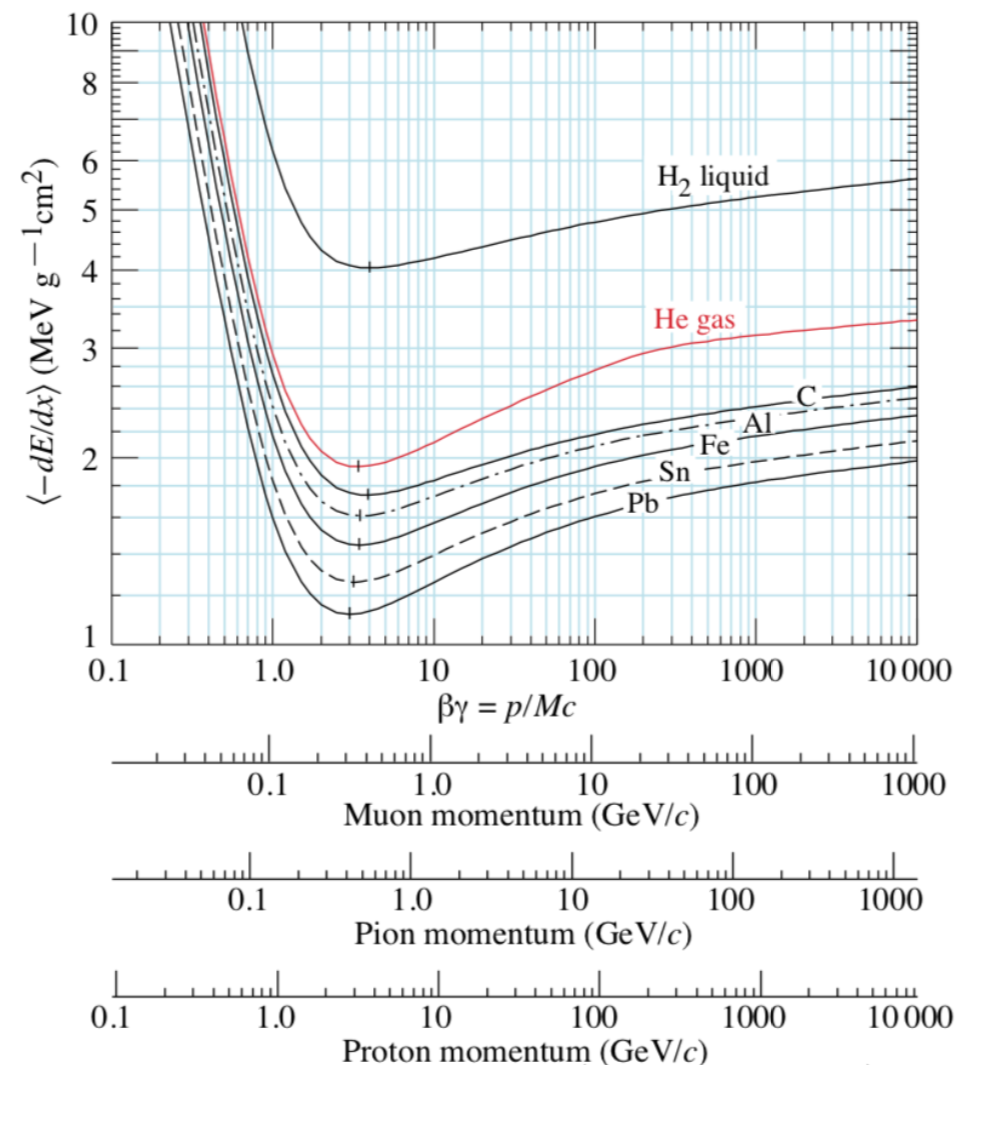
\includegraphics[width=\textwidth]{passRadMat12}
  \caption{Energy loss as a function of $\beta \gamma$, illustrating the relatively small variations of the position in $\beta \gamma$ of the minimum of ionization, and that curves are very similar. The correspondence in terms of momentum with $\beta \gamma$ for different particles is also given.}
  \label{fig:passRadMat12}
\end{figure}

Since the energy loss reaches its maximum for low $\beta$, if the absorber is deep enough, the maximum amount of released energy will be close to the stopping point of the particle.

The dependence of Bethe-Bloch formula on the incoming particle mass and charge allows, as shown in figure \ref{fig:passRadMat13}, the identification of different kind of particles. This property has been crucial in the past, allowing classification and discovery of elementary particles.

\begin{figure}
  \centering 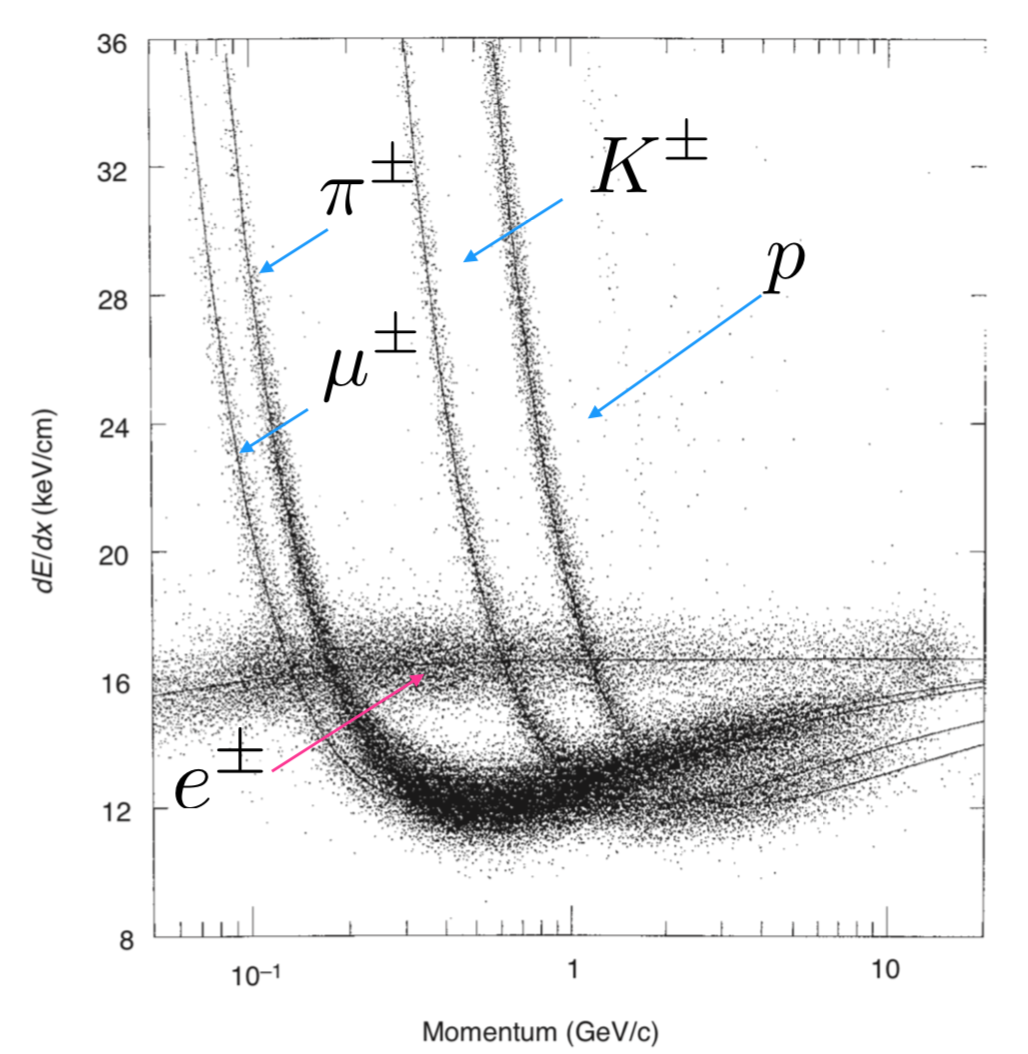
\includegraphics[width=\textwidth]{passRadMat13}
  \caption{The measured energy loss from different particles as a function of their momentum, illustrating the discriminating power of the ionization energy loss measurements -- combined with  momentum measurements -- to identify particles.}
  \label{fig:passRadMat13}
\end{figure}
%%% Local Variables:
%%% mode: latex
%%% TeX-master: "../book"
%%% End:

\subsection{Orders of magnitude} 
The Bethe-Bloch formula allows us to answer a fundamental experimental question: why do \(\alpha\), \(\beta\) and \(\gamma\) radiation travel with so different ranges in matter? We will use Fig.~\ref{fig:passRadMat12} to provide a quantitative answer.

We know that \(\alpha\) particles are helium nuclei, i.e. their mass is \(m_\alpha\approx4m_p=\SI{3.7}{GeV}\) and their charge is $+2e$. The typical energy -- \emph{kinetic} energy -- of \(\alpha\) particles is of a few \si{MeV}. As the \(\alpha\) particle is relatively heavy, \SI{5}{MeV} of kinetic energy correspond for example to
\[\beta\gamma = \frac{pc}{mc^2} = \frac{\sqrt{(T+mc^2)^2-(mc^2)^2}}{mc^2} = \frac{\sqrt{T^2+2mc^2T}}{mc^2} \approx 0.05.\]
An $\alpha$ particle will therefore be in the part of the Bethe Bloch formula in which the energy loss is high; its charge is twice as much as the electron charge, which brings  a factor four higher energy loss. Depending on the material, its energy loss normalised to the material density will be of about \SI{8}{MeV/gcm^2}, which leads to a range of a few \si{cm} in air, and about \SI{20}{\micro m} in water. This is consistent with the experimental evidence for which \(\alpha\) radiation can be easily stopped with a thin paper layer.

In the case of $\beta^-$ and $\beta^+$ radiation, i.e. electrons and positrons with $m_e=\SI{511}{keV}$, the typical energies depend on the decaying nucleus and are between a few \si{keV} to about \SI{1}{MeV}. An electron with \SI{500}{keV} of kinetic energy from \(^{40}K\) decays will for example have \(\beta\gamma\approx2\), close to the minimally ionising particle regime; while an electron with \SI{100}{keV} from \(^{60}Co\) decays will have \(\beta\gamma\approx0.7\), with almost a factor \(3\) higher energy loss per \si{cm}.
Experimentally, a thin aluminium foil is usually enough to absorb $\beta$ radiation.

As for $\gamma$ radiation, i.e. massless photons with energies between a few \si{keV} to a few \si{MeV} (or, in the case of X rays, between about \SI{100}{eV} and a few \si{keV}), the energy loss mechanisms are described in detail in the following sections. One should note that photons can induce ionisation indirectly, via the photoelectric effect and Compton effect. We anticipate that the typical range of $\gamma$ radiation in matter is higher than for $\alpha$ and $\beta$ radiation, and can reach a few \si{km} in air: long, high-density absorbers (e.g. lead) must be used in order to safely stop $\gamma$ radiation.
 
\subsection*{Take-home lessons}
\begin{itemize}
    \item  Charged particles lose their energy, when interacting with matter, due to ionisation or excitation of other atoms, to Coulomb scattering with atomic nuclei or to radiation emission in the field of atomic nuclei (\emph{bremsstrahlung}). Photons instead undergo photoelectric effect, Compton scattering and electron-positron pair production.
    \item The atomic model by Niels Bohr assumes a hydrogen atom to be composed of a proton and an electron, kept together by the Coulomb potential. The mass of the proton is assumed to be much greater than the mass of the electron, and the atom is assumed to be stationary, i.e. electrons revolve in stationary, circular orbits around the nucleus without radiating energy. Angular momentum is conserved and is assumed to be quantised in units of $\hslash$: as a result, the energy and radius of each orbits are quantised (in agreement to the experimental observations). This model is often sufficient to calculate with good accuracy the energy loss of particles interacting with matter.
    \item In Bohr's model, a particle which travels close to an atom with velocity $v$ receives a change in momentum ("momentum transfer") due to the Coulomb interaction between the particle and atomic electrons. The momentum transfer is only in the directional orthogonal to the direction of the particle, and is equivalent to having an  "average force" -- independent on time -- applied at a distance equal to the impact parameter $b$, for a time $2b/v$ ("scattering time"). This calculation assumes the electron orbit to be a straight line, an assumption which is accurate only when $v$ is significantly larger than the orbital velocity of the electron. One can derive, in the non-relativistic approximation, the energy loss of the incoming particle as a function of its impact parameter. By combining this quantity with the number of electrons along the path of the particle, one can calculate the average energy loss per element path length, $\od{E}{x}$: it is however necessary to know the minimum and maximum impact parameter values of the particle. The minimum value can be taken from the indetermination principle as the $b_\text{min}=\Delta x \approx \hslash/p_e$, where $p_e$ is the momentum of the electron; the maximum value can instead be taken from the fact that the scattering time should be less than the period of the electron orbit, and correcting the resulting value for relativistic time dilation effects. As a result, one gets Bohr's formula, which is able to describe energy loss of a particle in a medium with reasonable accuracy over a limited kinematic range.
    \item The Bethe-Bloch formula comes from a more accurate calculation of energy loss, based on a quantum mechanical approach which is also extended in the relativistic regime. Again, the main task is to express the energy transfer as a function of the impact parameter -- the higher the first, the lower the second. The maximum energy transfer depends on the mass of the electron, the mass of the particle and its velocity, and can often be approximated as $\Delta E_\text{max} = 2m\beta^2\gamma^2c^2$. The mimimum energy transfer instead depends on the average ionisation energy of the atom, which is proportional to its atomic number ($\langle I\rangle\propto Z$). The Bethe-Bloch formula is often expressed in terms of the energy loss per unit path length normalised to the density of the material, $\frac{1}{\rho}\od{E}{X}$, which does not depend strongly on the material.
    \item The complete calculation of the Bethe-Bloch energy loss shows three different regimes. When the incoming particle is very slow (low $\beta\gamma$), it loses energy as $1/\beta^2$.  The energy loss $\frac{1}{\rho}\od{E}{X}$ then reaches a minimum for $\beta\gamma\approx3\div3.5$, corresponding to about \SI{2}{MeV g/cm^2} (\emph{minimally ionising particle}). Then, the energy loss rises with $2\ln(\beta\gamma)$, due to the fact that the electic field seen by the incoming particle is increased by the Lorentz boost. For very low $\beta\gamma$ the calculation is not correct, and empirical models must be used; for very high $\beta\gamma$, radiative effects (bremmstrahlung) become dominant and the energy loss from ionisation starts becoming negligible. Two corrections are included, the \emph{density effect} for high $\beta\gamma$ (the electric field is screened due to polarisation of the medium) and the \emph{shell correction} for low $\beta\gamma$ (slow particles aren't much faster than electrons).
    \item The cross-section of the ionisation energy loss can be obtained from the Bethe-Bloch formula, and is inversely proportional to the energy loss: collisions with high energy loss are therefore less probable than those with low energy loss.
    \item The Bethe-Bloch calculation gives the \emph{average} energy loss. Since energy loss is a stochastic process, in real life one needs to take into account the thickness of the material the particle travels in. In thick materials, one can assume that the energy loss is due to a sequence of collisions in which only a small fraction of the energy of the particle is lost: one can therefore apply the central limit theorem and calculate the mean and standard deviation of the distribution of energy loss, when density effect and shell correction are neglected. In the limit of very thin materials, one cannot apply the central limit theorem and fluctuations in the energy loss will follow a Landau distribution, which has a most probable value lower than the average energy loss from the Bethe-Block formula.
    \item The \emph{range} of a particle in a medium is defined as its mean path before it loses all its kinetic energy. Its experimental curve is smeared (due to straggling) with respect to an ideal integration of the energy loss per unit path length.
    \item By comparing the \od{E}{x} of different particles, one may deduce their mass and charge, and \emph{perform particle identification}.
    \item Depending on the angle at which a particle travels in a medium, it may be \emph{channeled} in a path in which the number of encountered electrons is lowered than the average. This phenomenon happens for small incident angles, $\approx \SI{1}{deg}$, and $\beta\approx0.1$.
\end{itemize}
\section*{Questions}
\begin{itemize}
    \item 
\end{itemize}